\documentclass{article}


\usepackage{pgfplots}
    \pgfplotsset{compat=1.17}
\usepackage{graphicx}
    \graphicspath{{./images/}}
\usepackage{amsmath}

\title{Problem Solving and Modelling Task}
\author{Alexander Arthur}



\begin{document}

\maketitle
\setcounter{tocdepth}{1}
\tableofcontents

\section{Introduction}
    The given task is to predict the time period after which a population of bacteria will completely cover the surface of the water in a dam (Figure \ref{figDamOutline}). In order to do this, the area of the lake must first be calculated from the diagram provided. Once this area is known, the growth of the bacteria can then be projected and the point at which the lake will be covered subsequently found.

    \begin{figure}
        \centering
        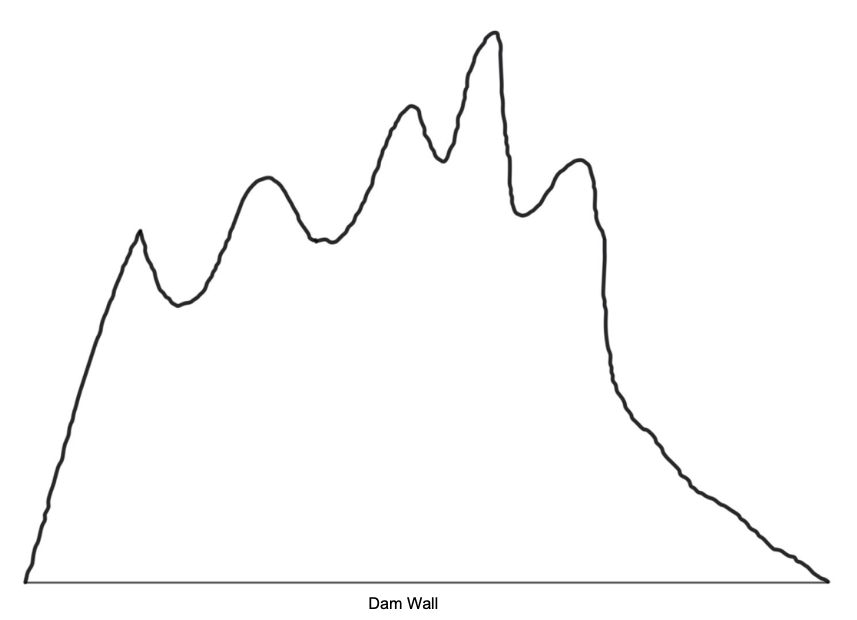
\includegraphics[width = 12cm]{damDiagram.png}
        \caption{Diagram of outline of dam}
        \label{figDamOutline}
    \end{figure}



\section{Assumptions and observations}

    \subsection{Observations}

    When the diagram of the dam is oriented with the straight wall colinear to the $x$-axis, the rest of the outline passes the vertical line test, meaning that it can be modelled with some sort of mathematical function.

    % Need second observation (issue #1)    
    
    \subsection{Assumptions}
    
    In order to simplify the problem, certain assumptions must be made either due to a lack of information provided or to bring the scope of the problem to a reasonable scale.

    Should the water level of the dam change, this would change the water's surface area, since it is unlikely the walls of the dam are perfectly vertical. Changing the surface area of the dam would in turn affect the point at which the bacteria would cover the entire lake, affecting the result of the investigation. Since no data is provided on the water level, it is reasonable to assume that it is static, and will not have any effect on the surface area of of the lake.

    In a similar vein, there are many factors which can influence the growth rate of a population of bacteria, including access to a food source, temperature and competition for space. Similarly to the dam's water level, no data is provided around this, meaning that it must be assumed that the none of these factors will affect the bacteria as the population grows.
    
\section{Translation of mathematical concepts}

    As per the requirements of the task, a mathematical approach must be used to calculate the area of the dam. To satisfy this requirement, the definite integral of a piecewise function will be used to calculate the area of dam.

    In statistical modelling, a model can be overfitted to a dataset such that it is highly accurate within the domain of the data, but is wildly inaccurate outside this domain, meaning that it cannot be used to predict values outside the domain of the data and therefore is not useful. However, in this task, for any given segment of the piecewise function the only domain which is applicable is that of that segment, meaning that the concept of the function being over-fitted does not apply. In addition, the Weierstrass approximation theorem states that for any continuous function $f$ over the real interval $[a, b]$ and any $\epsilon > 0$ there exists a polynomial $p$ such that $|f(x) - p(x)| < \epsilon$, where $a \leq x \leq b$.
 
    This means that since the only key metric used to select a function is its accuracy within the specified domain, regression was used to select a function within each defined section, and the regression models used were strictly polynomial; the degree of the polynomial was simply increased until the function fit the data to a sufficient degree of accuracy ($R^2 > 0.97$).

    To generate the points to be used for these regressions, a Python script was written to list the coordinates of the topmost black pixel in each column of pixels. This generated a list of 1262 pixel coordinates, which were scaled to the dimensions of the dam such that one unit on the $x$ and $y$ axes were each equal to 1 meter and subsequently used to generate regression models (Figure \ref{figRawData}).

    \begin{figure}
        \centering
        \begin{tikzpicture}
            \begin{axis}[
                    title = {\textbf{Raw data points}},
                    xmajorgrids = true,
                    ymajorgrids = true
                ]
                \addplot[only marks, mark = x]table[x=x, y=y]{data.txt};
            \end{axis}
        \end{tikzpicture}
        \caption{Raw data from Python script}
        \label{figRawData}
    \end{figure}

    In an ideal scenario, a single function could be used to model the entire length of the dam's outline. However, due to the computational limits of the available software a polynomial regression of sufficiently high degree is not possible. This means that the data was instead divided into several sections (Figure \ref{figSectionedData}), each of which were then  used to run a polynomial regression. Since these sections were selected to have more simple shapes than the entire dataset, polynomials of much lower degree ($< 6$) were sufficient to replicate their shape to a sufficient degree of accuracy.

    \begin{figure}
        \centering
        \begin{tikzpicture}
            \begin{axis}[
                    title = {\textbf{Sectioned data}},
                    xmajorgrids = true,
                    ymajorgrids = true
                ]
                \addplot[only marks, mark = x, color = red]table[x=x1, y=y1]{data/section1.txt};
                \addplot[only marks, mark = x, color = blue]table[x=x2, y=y2]{data/section2.txt};
                \addplot[only marks, mark = x, color = red]table[x=x3, y=y3]{data/section3.txt};
                \addplot[only marks, mark = x, color = blue]table[x=x4, y=y4]{data/section4.txt};
                \addplot[only marks, mark = x, color = red]table[x=x5, y=y5]{data/section5.txt};
                \addplot[only marks, mark = x, color = blue]table[x=x6, y=y6]{data/section6.txt};
                \addplot[only marks, mark = x, color = red]table[x=x7, y=y7]{data/section7.txt};
                \addplot[only marks, mark = x, color = blue]table[x=x8, y=y8]{data/section8.txt};
            \end{axis}
        \end{tikzpicture}
        \caption{Data shown in coloured sections}
        \label{figSectionedData}
    \end{figure}

\subsection{Calculation of area}

    Let us define a variable $b$ for the boundaries between the sections, such that $b_0 = 0$, $b_1 = 4.3$ \ldots $b_8 = 30$. Let us also  define the piecewise function $f$ as follows:

    \begin{equation}
        f(x) = \begin{cases}
            f_1(x) & b_0 \leq x < b_1 \\
            f_2(x) & b_1 \leq x < b_2 \\
            \vdots & \vdots \\
            f_7(x) & b_6 \leq x < b_7 \\
            f_8(x) & b_7 \leq x \leq b_8
        \end{cases}
        \label{eqnPiecewiseFunction}
    \end{equation}

    The subfunctions $f_1 \cdots f_8$ were found using polynomial regression models and are defined as follows:

    \begin{align*}
        f_1(x) &= -1.2364x^2 + 25.667x - 1.4657 \\
        f_2(x) &= 0.0922x^5 - 3.4033x^4 + 47.748x^3 - 315.07x^2 + 968.69x - 1022.9 \\
        f_3(x) &= -0.4898x^4 + 22.736x^3 - 388.82x^2 + 2903.4x - 7897 \\
        f_4(x) &= 1.1895x^6 - 110.38x^5 + 4255.2x^4 - 8.7230\cdot 10^04x^3 + 1.0027\cdot 10^6x^2 \\ &- 6.1276\cdot 10^6x + 1.5551\cdot 10^7 \\
        f_5(x) &= 6046.8x^6 - 6.5135 \cdot 10^5x^5 + 2.9233 \cdot 10^7x^4 - 6.9967 \cdot 10^8x^3 \\ &+ 9.4192 \cdot 10^9x^2 - 6.7624 \cdot 10^{10}x + 2.0228 \cdot 10^{11} \\
        f_6(x) &= -3.4000x^3 + 199.63x^2 - 3897.0x + 25388 \\
        f_7(x) &= 253.31x^5 - 26978x^4 + 1.1491 \cdot 10^6x^3 - 2.4471 \cdot 10^7x^2 + 2.6052 \cdot 10^8x \\ &- 1.1093 \cdot 10^9 \\
        f_8(x) &= -0.0556x^3 + 4.6621x^2 - 134.73x + 1347.2
    \end{align*}

    \begin{figure}
        \centering
        \begin{tikzpicture}
            \begin{axis}[
                    title = {\textbf{Function modelling outline of lake}},
                    xmajorgrids = true,
                    ymajorgrids = true,
                    restrict y to domain*=0:140
                ]
                \addplot[color = red, domain = 0:4.278922345, smooth]{-1.23638*x^2 + 25.66721*x - 1.46574};
                \addplot[color = blue, domain = 4.278922345:11.07765452, smooth]{0.0922*x^5 - 3.4033*x^4 + 47.7479*x^3 - 315.0713*x^2 + 968.6939*x - 1022.9268};
                \addplot[color = red, domain = 11.07765452:14.38193344, smooth]{-0.4898*x^4 + 22.7361*x^3 - 388.8167*x^2 + 2903.3720*x - 7896.9865};
%                \addplot[color = blue, domain = 14.38193344:17.49603803, smooth]{3.4624*x^5 - 280.3803*x^4 + 9065.4212*x^3 - 146281.0500*x^2 + 1177965.4248*x - 3786937.4387};
                \addplot[mark = none, color = blue, smooth]table[x=x4, y=y4]{data/calculatedSection4.txt};
                % 6046.771999329330000*C2^6 - 651353.151682996000000*C2^5 + 29232785.773414700000000*C2^4 - 699672004.563012000000000*C2^3 + 9419179590.356580000000000*C2^2 - 67624182395.647400000000000*C2 + 202279215616.422000000000000
                \addplot[mark = none, color = red, smooth]table[x=x5, y=y5]{data/calculatedSection5.txt};
                % 3.4000047417*E3^3 + 199.6280602865*E3^2 - 3,897.0360743426*E3 + 25,388.8275429106
                \addplot[mark = none, color = red, domain = 18.42313787:20.681458, smooth]{-0.000296363*x^3 + 0.731989*x^2 -601.112*x + 164741 };
            \end{axis}
        \end{tikzpicture}
        \caption{Piecewise function modeling the outline of the dam}
        \label{figDamModel}
    \end{figure}

    \begin{equation}
       A = \sum_{r=1}^8 \int_{x_{r-1}}^{x_r} f_r(x)\ {dx}
    \end{equation}


%   Since we are not trying to make predictions outside the domains of the relevant sections, the type of function used to model them is not relevant as long as it is a close enough fit within the domain. Since any function can be expressed as a polynomial of infinte degree, in this situation it is reasonable to only use polynomial models and simply increase their degree until they fit the data sufficiently closely, namely an $R^2$ of at least [R SQUARED]

\end{document}
